\documentclass{article}

% arXiv recommended packages
\usepackage[utf8]{inputenc}
\usepackage[T1]{fontenc}
\usepackage{hyperref}
\usepackage{url}
\usepackage{booktabs}
\usepackage{amsfonts}
\usepackage{nicefrac}
\usepackage{graphicx}
\usepackage{xcolor}
\usepackage{amsmath}
\usepackage{amssymb}
\usepackage{algorithm}
\usepackage{algorithmic}
\usepackage{natbib}
\usepackage{caption}
\usepackage{subcaption}

% Page setup for arXiv
\usepackage[margin=1in]{geometry}

% Draft helper — strip before submission
\newcommand{\todo}[1]{\textcolor{red}{[TODO: #1]}}

\title{TrackFM: A Foundation Model for Vessel Trajectory Forecasting}

\author{
  Paul Singerman\thanks{Corresponding author: pgs16@psu.edu} \\
  Penn State University\\
  \texttt{pgs16@psu.edu}
  \and
  Dennis Murphy \\
  Penn State University\\
  \texttt{djm6391@psu.edu}
  \and
  Carson Forsyth \\
  Penn State University\\
  \texttt{cpf5502@psu.edu}
}

\date{}

\begin{document}

\maketitle

\begin{abstract}
We present TrackFM, a foundation model for vessel trajectory forecasting
trained on 26 months of Danish Automatic Identification System (AIS) data
(7.1B positions, 45{,}469 vessels). TrackFM is a decoder-only causal
transformer that outputs full probability densities over future position via
a spectral density head, pretrained by multi-horizon next-position
prediction. We depart from prior work in three ways. First, we evaluate
forecasts operationally: the area a searcher must cover to contain the
vessel with 90\% probability, rather than loss ratios against dead
reckoning. Second, we introduce a \emph{horizon-scaled} output canvas whose
physical extent grows with the reachable set, letting one model forecast
every vessel at every horizon: at two hours it contains 90\% of vessels
within 35\,km\textsuperscript{2} while covering the 19\% of fast movers
that fixed-canvas models structurally censor. Third, we show that a single
hidden layer inside the density head---a projector, in the self-supervised
learning sense---is the largest single quality lever, reducing two-hour
containment area by 33--39\% and improving representation transfer by
18--25\%. The pretrained representations transfer to
811-way destination prediction (beating an origin-conditioned lookup at
every top-$k$), arrival-time regression, and 15-class vessel-type
classification, where every comparison includes random-initialization and
na\"ive-baseline controls: pretraining roughly doubles linear-probe quality
over a random encoder across tasks. Counter to scaling intuition, an
18M-parameter model matches or beats a 116M-parameter one on forecasting
and classification transfer at our pretraining budget, while capacity pays
only on regression transfer. We release code, models, and the uniform
evaluation harness.
\end{abstract}

\section{Introduction}

The maritime industry forms the backbone of global trade, with over 80\% of
international goods transported by sea \citep{unctad2023}. The Automatic
Identification System (AIS) broadcasts vessel positions, speeds, and courses
continuously, and effective use of this data stream underpins maritime
safety, search and rescue, port operations, and security applications.

The operational question a forecasting system answers is rarely ``what is
the expected position?'' but ``\emph{where should we look?}'' A search
asset, a port scheduler, or a collision-avoidance system needs a region
that contains the vessel with high probability, and the cost of the
forecast is the size of that region. We therefore evaluate probabilistic
trajectory forecasts by \emph{containment area}: the area of the smallest
predicted-density region that captures the true position with 90\%
probability. This metric exposes failure modes that likelihood ratios hide,
and it makes population coverage explicit---a model that only produces
forecasts for slow vessels cannot hide behind averages.

Forecasting over multiple horizons with one model raises a geometry
problem. A vessel's reachable set grows with lead time: a canvas sized for
15-minute forecasts censors fast vessels at two hours, while a canvas sized
for two hours wastes resolution at 15 minutes. Prior trajectory models fix
the output geometry as an architectural constant and inherit one of these
failure modes. We instead scale the output canvas with the physical
reachable set, $R(t) = r_0 + v_{\max} t$, so the model forecasts
\emph{every} vessel at \emph{every} horizon on a canvas that is always
appropriately sized, and the canvas bound is a physical constant rather
than a tuned hyperparameter.

Finally, we treat forecasting as pretraining for a \emph{foundation model}
\citep{devlin2019bert, brown2020gpt3, radford2021clip}: the same frozen
encoder should transfer to destination prediction, arrival-time estimation,
and vessel classification. We take the ``foundation'' claim seriously
methodologically---every transfer result is reported against a
random-initialization encoder control and a task-appropriate na\"ive
baseline, at every adaptation budget (linear probe, probe-then-finetune,
full finetuning).

Our contributions:
\begin{enumerate}
    \item \textbf{Operational evaluation}: containment area at fixed
    capture probability, computed by one uniform harness across all models
    and eras, with the evaluation frame and covered population stated for
    every comparison.

    \item \textbf{Horizon-scaled forecasting geometry}: a reachable-set
    canvas that covers 100\% of vessels at every horizon. At two hours it
    achieves 35\,km\textsuperscript{2} p90 containment on the full
    population, within 8\% of a wide fixed-canvas specialist while
    dominating it at 15--60 minutes by $2$--$3\times$, and removing canvas
    size from the hyperparameter space entirely.

    \item \textbf{The head projector effect}: one hidden layer between
    encoder and density coefficients cuts two-hour containment by
    33--39\% \emph{and} improves frozen-feature transfer by 18--25\%---the
    same projector phenomenon documented in contrastive SSL, appearing in
    a generative-density pretraining objective.

    \item \textbf{A controlled transfer suite}: 811-way port-destination
    (with privileged-lookup baselines), arrival-time regression, and
    15-class vessel type over 677k windows with vessel-disjoint splits;
    random-init and na\"ive baselines at every rung. Pretraining
    approximately doubles linear-probe quality across tasks; full
    finetuning erases architecture differences, isolating where
    representation quality actually matters.

    \item \textbf{Scale findings that inform deployment}: at a 50M-sample
    budget, 18M parameters match 116M on forecasting and classification
    transfer (capacity pays only on regression), and a grid-free
    physical-spectrum head variant ties for best transfer while trailing
    on containment---head choice and backbone quality dissociate.
\end{enumerate}

\section{Related Work}

\paragraph{Deep Learning for Trajectory Prediction}
Recurrent neural networks, particularly LSTMs, have been widely applied to
vessel trajectory prediction \citep{nguyen2018geotracknet}. Transformer
architectures capture longer-range temporal dependencies: TrAISformer
\citep{nguyen2021traisformer} introduced a sparse high-dimensional AIS
representation with classification loss to handle multimodality; TRFM-LS
\citep{jiang2023trfmls} combined transformers with LSTM modules; TPTrans
\citep{wang2024tptrans} employed multi-head attention for spatiotemporal
features. Graph neural networks model vessel interactions
\citep{zhao2022kgcnlstm, wang2024stmgf}. Our work differs in evaluating
probabilistic forecasts by operational containment area rather than
point-estimate error, and in treating the forecaster as a pretrained
backbone for transfer.

\paragraph{Foundation Models for Trajectories}
TrajFM \citep{lin2024trajfm} targets vehicle trajectories with masking and
recovery objectives; the Pretrained Mobility Transformer \citep{jiang2024pmt}
applies GPT-style pretraining to human mobility; time-series foundation
models address prediction and anomaly detection broadly \citep{jin2024tsfm}.
Maritime trajectories differ in continuous unconstrained space, irregular
sampling, and reachable sets that grow with horizon---the property our
horizon-scaled geometry exploits.

\paragraph{Maritime Behavior Analysis}
Anomaly detection taxonomies and methods are surveyed in
\citet{riveiro2018anomaly}; deep approaches include autoencoders and GANs
\citep{chen2024wgananomalym} and multi-task frameworks \citep{shin2025aisllm}.
Collision risk work increasingly integrates probabilistic trajectory
prediction \citep{zhang2025collisionrisk}, which requires exactly the
calibrated spatial densities TrackFM outputs.

\section{Data}

We use the complete Danish Maritime Authority AIS feed for the Danish
maritime zone (54--58.5$^\circ$N, 7--16$^\circ$E) from January 2023 through
February 2025: \textbf{788 days, 7.14B positions, 3.11M track segments,
45{,}469 distinct vessels}---an order of magnitude more data than our
earlier 69-day study. Cleaning (bounding box, speed-outlier removal,
4-hour-gap segmentation, transponder-collision splitting) and windowing
yield 168.7M training windows; each window is a 128-position input section
followed by an 800-position forecast section ($\approx$2.6\,h). Splits are
temporal (80/10/10); all model selection uses the validation period, and
the vessel-classification task additionally uses vessel-disjoint splits.
Every observation is the 6-vector
$(\phi, \lambda, v, \sin\theta, \cos\theta, \Delta t)$: normalized
latitude/longitude, speed over ground, course encoded on the circle, and
inter-report interval. Pretraining runs in this paper consume a uniform
50M-sample budget (38\% of training windows) so that architecture
comparisons are compute-matched; the released flagship model trains on the
full corpus. \todo{flagship numbers when trained}

\section{Model}

\subsection{Backbone}
TrackFM is a decoder-only causal transformer: inputs are linearly projected
to $d_{\text{model}}$, combined with positional encodings, and processed by
$L$ pre-norm layers under a causal mask. The backbone is deliberately
standard; the contributions of this paper live in the output geometry, the
density head, and the evaluation.

\begin{table}[t]
    \centering
    \caption{Model scales. The champion configuration is \textbf{Large};
    at our pretraining budget XLarge does not improve forecasting
    (Section~\ref{sec:scale}).}
    \label{tab:model_scales}
    \begin{tabular}{lccccc}
        \toprule
        Scale & $d_{\text{model}}$ & Heads & Layers & FFN & Params \\
        \midrule
        Small & 128 & 8 & 4 & 512 & $\sim$2M \\
        Large & 384 & 16 & 8 & 2048 & $\sim$18M \\
        XLarge & 768 & 16 & 16 & 3072 & $\sim$116M \\
        \bottomrule
    \end{tabular}
\end{table}

\subsection{Multi-horizon conditioning}
A single backbone pass yields hidden states for every position; forecasts
at arbitrary lead times are produced by conditioning the density head on a
sinusoidal encoding of the cumulative elapsed time $\tau$ to the target.
Training samples multiple horizons per position (uniform over 1--800
steps), and causal subwindow training turns every position of every window
into a training example, extracting roughly $30\times$ more signal per
batch than fixed input/output splits. A leak test (perturbing future inputs
under the causal mask) verifies no information leakage.

\subsection{Horizon-scaled output canvas (``cone'')}
\label{sec:cone}
The density head rasterizes onto a $G \times G$ canvas ($G{=}64$) spanning
$\pm R$ degrees around the vessel's current position. Fixed-canvas models
choose $R$ once, architecturally. We instead set, per forecast,
\begin{equation}
    R(t) \;=\; r_0 + v_{\max}\, t,
\end{equation}
a linear reachable-set bound with $r_0 = 0.02^{\circ}$ and $v_{\max}$ the
99.9th-percentile effective vessel speed measured from the corpus
($1.71\times10^{-4}$\,deg/s $\approx$ 37\,kn). Targets are normalized by
$R(t)$, so the loss is scale-free; the canvas is $\pm0.03^{\circ}$ at one
minute and $\pm1.25^{\circ}$ at two hours. Every vessel is inside the
canvas at every horizon by construction---coverage is a property of the
geometry, not a hope about the data distribution.

\subsection{Density heads}
\label{sec:heads}
The head maps the conditioned hidden state to coefficients of a 2D Fourier
basis on the canvas; a softmax over the synthesized $G^2$ logits yields a
proper density. The loss is cross-entropy against a Gaussian soft target
($\sigma$ scaled to the canvas). We study three head families:

\textbf{Linear} (prior work): a single linear map to the $2(2F{+}1)^2$
coefficients ($F{=}12$).

\textbf{Projector (``mlp'')}: one hidden layer
(Linear--GELU--Linear, width $d_{\text{model}}$) before the coefficient
map. This is the paper's single largest quality lever
(Section~\ref{sec:projector}).

\textbf{Physical spectrum}: a grid-free variant that indexes coefficients
by \emph{physical} frequency $k_j = j/2R(t)$ and evaluates a learned
continuous spectrum $\varphi(\gamma(k), h)$ at each harmonic, making
scale-equivariance exact by construction (slot $j$ at canvas $R$ equals
slot $2j$ at $2R$ analytically). It trails the projector head on
containment while matching the best models on representation transfer
(Section~\ref{sec:spectrum}).

\section{Evaluation: containment area, uniformly}
\label{sec:metric}

For each forecast we sort predicted cell probabilities and report the rank
of the true cell at the 90th percentile of the evaluation population
(p90 rank), converted to km\textsuperscript{2}. To compare models with
different native canvases fairly, all densities are re-binned onto a common
evaluation frame with fixed \textbf{0.6\,km\textsuperscript{2} physical
cells}; unless stated otherwise the frame is $\pm0.3^{\circ}$ around the
current position and the split is validation. Every number in this paper
comes from \emph{one} harness pass at \emph{one} metric version---we never
mix historical training-time curves into comparisons. Two protocol rules
proved essential and we adopt them as reporting standards:
(1) every table states its evaluation \emph{frame} and the \emph{fraction
of the population} that frame admits; (2) dead-reckoning and last-position
nulls are scored under the identical harness as gates.

\section{Forecasting experiments}

\subsection{Main result: geometry $\times$ head}
\label{sec:georesults}

\begin{table}[t]
    \centering
    \caption{Containment (p90 rank in 0.6\,km\textsuperscript{2} cells;
    lower is better) on the $\pm0.3^{\circ}$ frame, validation split,
    50M-sample budget. \emph{Pop.} = fraction of vessels the model's
    canvas covers at 2h. Fixed $\pm0.3^{\circ}$ models censor 19\% of
    vessels at 2h; their 2h column is computed only over the 81\% they
    cover (their home metric).}
    \label{tab:geometry}
    \begin{tabular}{llccccc}
        \toprule
        Model (18M) & Head & 15m & 30m & 1h & 2h & Pop.@2h \\
        \midrule
        \textbf{cone (ours)} & \textbf{projector} & \textbf{4} & \textbf{8} & \textbf{27} & 58 & \textbf{100\%} \\
        cone & linear & 7 & 14 & 40 & 87 & 100\% \\
        fixed $\pm0.3^{\circ}$ & projector & 4 & 8 & 23 & \textbf{39} & 81\% \\
        fixed $\pm0.3^{\circ}$ & linear & 6 & 16 & 40 & 64 & 81\% \\
        fixed $\pm1.25^{\circ}$ & projector & 11 & 15 & 32 & 52 & 100\% \\
        fixed $\pm1.25^{\circ}$ & linear & 14 & 21 & 47 & 82 & 100\% \\
        \bottomrule
    \end{tabular}
\end{table}

Table~\ref{tab:geometry} is the core forecasting result. Three findings:

\textbf{(1) The narrow fixed canvas wins its home metric by censoring.}
The $\pm0.3^{\circ}$ projector model posts the best 2h number (39), but
only over the 81\% of vessels its box can represent; scored on the full
population in a wide frame it collapses to 852 (border-replicated density
for every escaped vessel)---a structural wall, not a modeling error.

\textbf{(2) The horizon-scaled canvas covers everyone at near-specialist
cost.} On the full-population strict-2h comparison (identical tracks,
$\pm1.2^{\circ}$ frame), the cone forecasts 90\% of \emph{all} vessels
within 84 cells vs.\ 78 for the wide-fixed specialist ($+8\%$), while
beating it $2$--$3\times$ at 15m--1h (4/8/27 vs.\ 11/15/32)---the wide
canvas pays its resolution tax at every short horizon.

\textbf{(3) The gap decomposes.} Strict-tolerance analysis
($|t - 2\mathrm{h}| \le 60$\,s) splits the cone-vs-narrow difference into a
coverage burden (22$\to$30 cells: the cost any full-coverage model pays for
representing fast vessels) and a multiplexing cost (30$\to$36: sharing one
band-limited basis across a 63$\times$ range of canvas scales). Sparse
AIS reporters inflate p90 by $\sim$40\% for every model; containment cost
concentrates in reporting sparsity, an operationally meaningful
segmentation.

\begin{figure}[t]
    \centering
    
\includegraphics[width=0.95\textwidth]{figures/coverage_story_2h.png}
    \caption{The coverage story at 2h. Fixed narrow canvases win their
    censored home metric and collapse on the vessels they exclude; the
    horizon-scaled canvas covers 100\% of vessels within 8\% of the wide
    specialist while dominating at shorter horizons.}
    \label{fig:coverage}
\end{figure}

\subsection{The projector effect}
\label{sec:projector}
Adding one hidden layer to the density head improves 2h containment by
33\% (cone: 87$\to$58) to 39\% (fixed: 64$\to$39) at 18M scale, larger
than any geometry or scale intervention we tested. A head-depth ladder on
frozen features shows the knee at depth one. The same intervention
improves \emph{frozen-feature transfer} by 18--25\% (Section~\ref{sec:transfer}),
mirroring the projector phenomenon in contrastive SSL: the hidden layer
absorbs objective-specific warping that would otherwise distort the
encoder representation. We conjecture this is why the effect appears in a
generative-density objective as well.

\subsection{Scale}
\label{sec:scale}
Under the compute-matched 50M budget, scaling the encoder from 18M to 116M
parameters does not improve cone forecasting (85 vs.\ 87 at 2h with linear
heads) and does not match the projector intervention (fixed: 116M-linear 52
vs.\ 18M-projector 39). The scaling series (2M$\to$116M, fixed geometry)
saturates by 18M on containment. Transfer shows the same saturation on
classification tasks but \emph{not} on regression
(Section~\ref{sec:transfer}). \todo{xlarge-cone-projector scaling cell +
LR-transfer study land this week; full-data flagship separately}

\subsection{Grid-free spectrum head}
\label{sec:spectrum}
The physical-spectrum head makes scale-equivariance analytic instead of
learned. It loses to the slot-indexed projector head on containment
(67 vs.\ 58 at 2h) with a diagnostic signature: on the model's own
horizon-scaled canvas both heads are horizon-\emph{flat}, and the entire
gap is a constant $+1$ native cell of blur at every horizon---the cost of
imposing smoothness in frequency on coefficient functions that oscillate
(a density peaked at displacement $\delta$ has coefficients with period
$1/\delta$ in $k$). Yet its \emph{encoder} ties for best-in-suite on
vessel-type transfer (Section~\ref{sec:transfer}): head choice and backbone
quality dissociate. Because it needs no grid retraining at new horizons,
we develop it as the extension path to beyond-2h forecasting.

\section{Transfer experiments}
\label{sec:transfer}

All transfer tasks are built from the same corpus with temporal splits;
vessel classification is additionally vessel-disjoint. Following the
foundation-model framing, \emph{every} figure and table includes (a) a
random-initialization encoder put through the identical adaptation recipe
and (b) a task-appropriate na\"ive baseline.
\todo{random-init LP-FT/full-FT and random-init ETA controls land this
week (CHAIN17); linear-probe controls are complete}

\subsection{Port destination (811 classes)}
Linear probes on frozen encoders reach 0.254 macro-F1 (fixed-projector)
vs.\ 0.095 for the random-init control ($2.6\times$) and 0.125 for a
nearest-port baseline. Against a \emph{privileged} baseline that memorizes
each vessel's origin$\to$destination distribution from training data
(top-1/3/5 accuracy .754/.878/.907), the best frozen encoders win at every
$k$ (.776/.899/.920) \emph{without} access to the origin label.
Probe-then-finetune lifts all encoders uniformly ($\sim$$+35\%$ relative,
ordering preserved); full finetuning reaches 0.364 and \textbf{erases the
geometry gap} (fixed .364 vs.\ cone .363)---architecture choices matter for
forecasting, not for adapted transfer, so geometry can be selected on
forecasting merits alone.

\begin{figure}[t]
    \centering
    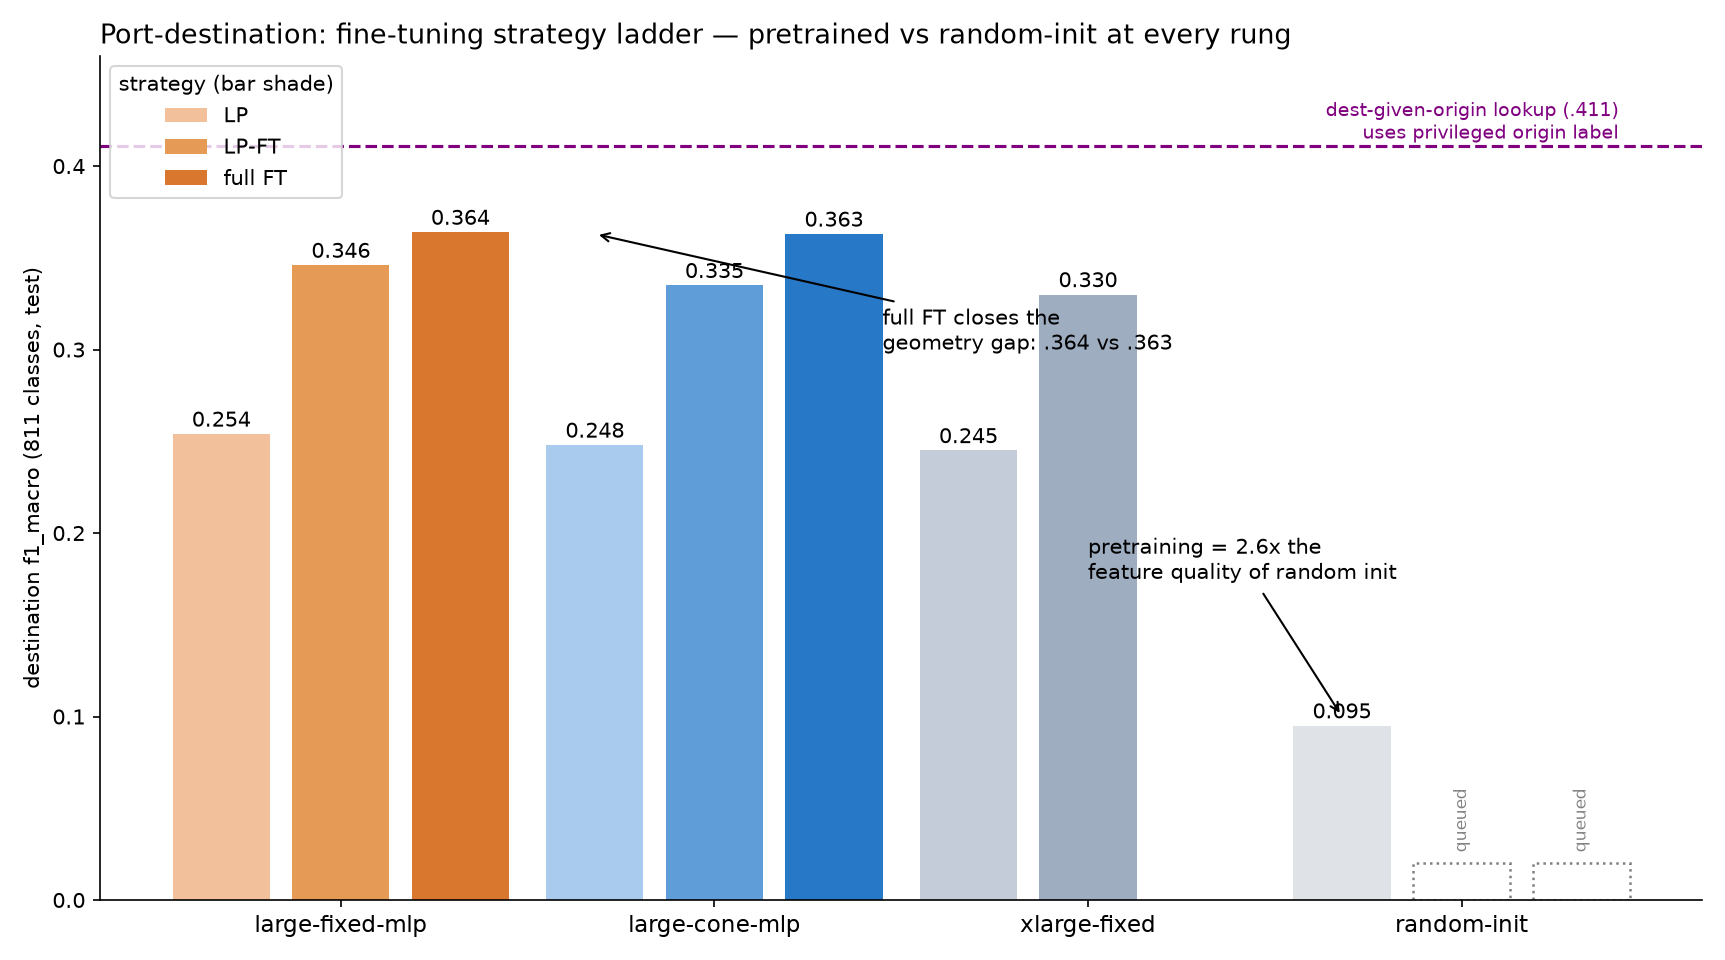
\includegraphics[width=0.9\textwidth]{figures/ft_strategy_progression.png}
    \caption{Adaptation ladder on port destination: linear probe $\to$
    probe-then-finetune $\to$ full finetuning, per encoder, with
    random-init control group and baselines.}
    \label{fig:ladder}
\end{figure}

\subsection{Arrival time (ETA)}
Linear-probe regression to remaining travel time: 505--544 minutes MAE
(medians 191--213), all beating the constant train-median baseline
(775/422) by $\sim$30--35\%. The encoder ordering \emph{reverses} relative
to classification: the 116M model is best, suggesting regression consumes
capacity that classification transfer saturates.

\subsection{Vessel type (15 classes, 677k windows)}
On vessel-disjoint splits, linear probes reach 0.383 macro-F1
(fixed-projector) and 0.382 (spectrum---the containment loser tying for
first), vs.\ 0.200 random-init, 0.151 kinematic-statistics, and 0.009
majority. All pretrained encoders clear the random control by wide
margins; modern projector-head encoders dominate our earlier-era 100M+
models. Notably, a geography-and-traffic \emph{conditioned} pretrain
variant improves forecasting ($-9\%$ containment) but \emph{degrades}
transfer ($-11\%$ F1 vs.\ its unconditioned sibling)---context channels
act as a crutch for the representation. We therefore keep the foundation
model unconditioned and treat context as a finetune-time addition.

\begin{figure}[t]
    \centering
    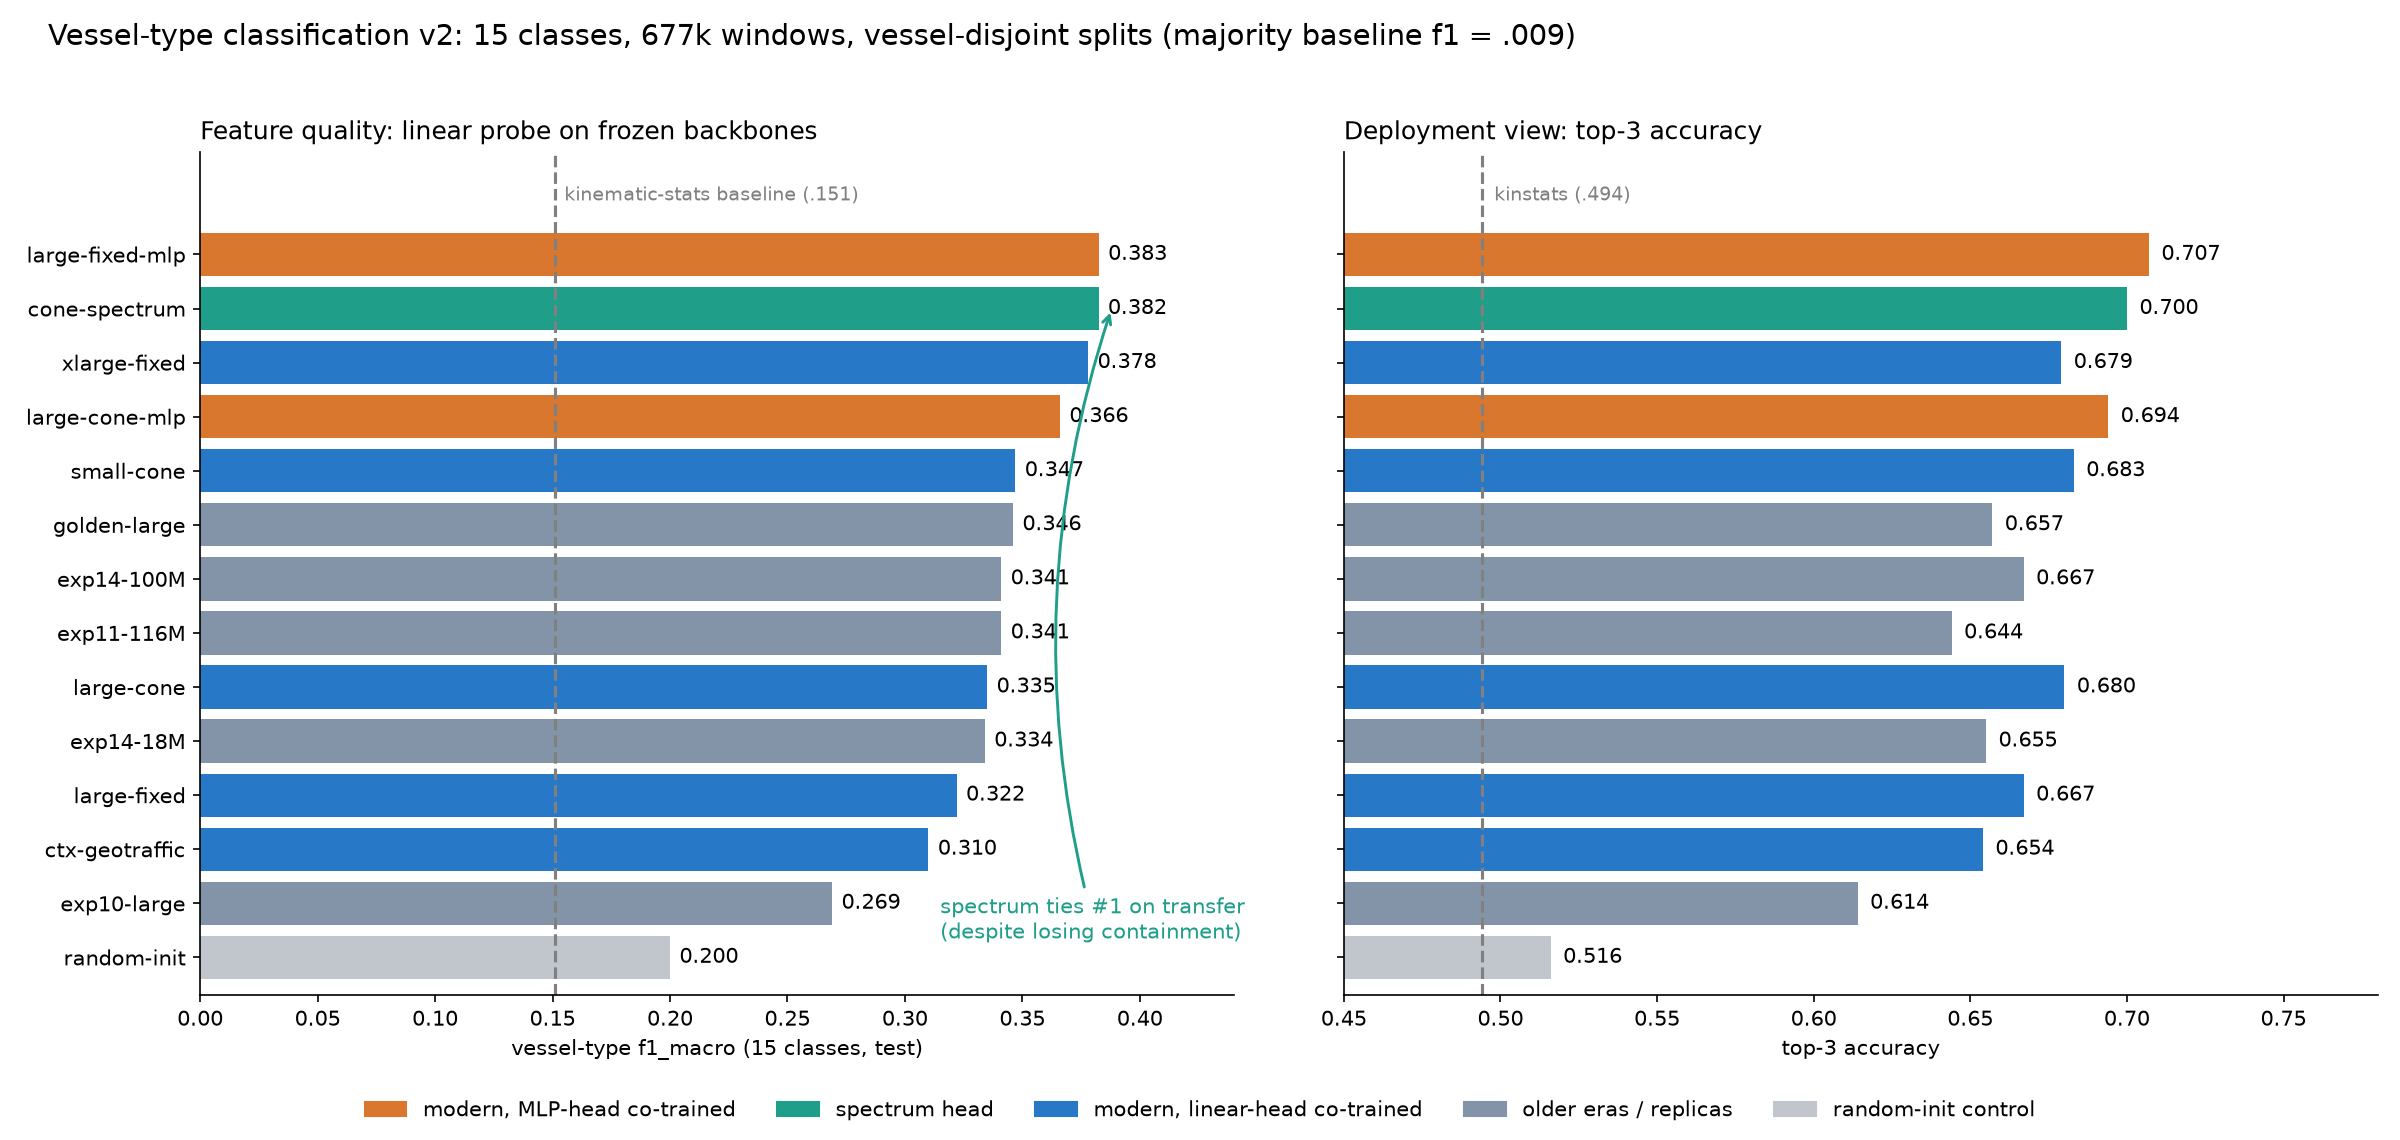
\includegraphics[width=\textwidth]{figures/ft_vessel_v2_leaderboard.png}
    \caption{Vessel-type linear probes: 14 encoders vs.\ random-init and
    na\"ive baselines. The spectrum-head encoder ties for first despite
    losing on containment---backbone quality and head quality dissociate.}
    \label{fig:vessel}
\end{figure}

\section{Discussion}

\paragraph{What makes the best pretrained forecaster?}
At realistic budgets the answer is not scale: it is output geometry
(coverage without resolution tax), head design (a projector layer), and
honest evaluation (containment over the full population). An 18M model
with the right head and geometry beats a 116M model without them on every
axis we measure except regression transfer.

\paragraph{Foundationness is a claim about controls.}
Pretraining roughly doubles frozen-feature quality over random
initialization across three tasks, survives probe-then-finetune with
ordering intact, and its representation advantages disappear exactly where
they should (full finetuning). The conditioned-pretraining result cuts the
other way---better forecasting, worse representations---showing the two
qualities can be traded and must both be measured.

\paragraph{Limitations.}
Single region (Danish waters); containment on sparse AIS reporters is
$\sim$40\% worse for all models; the full-data flagship and beyond-2h
horizons (via the grid-free head) are in progress; vessel interactions and
external context (weather, port state) are finetune-time extensions in the
current design. \todo{seed variance for headline FT comparisons if
reviewers require}

\paragraph{Broader impact.}
Improved maritime forecasting supports search-and-rescue, safety, and
environmental protection; the same capabilities could support surveillance.
We release models trained only on publicly available AIS broadcasts.

\section{Conclusion}
TrackFM shows that the best pretrained vessel forecaster at practical scale
comes from horizon-scaled output geometry, a projector density head, and
containment-based evaluation---not from parameter count---and that its
encoder transfers, with controls that make the foundation-model claim
falsifiable. We release code, the uniform harness, and pretrained models.

\section*{Acknowledgments}
AIS data was provided by the Danish Maritime Authority.

\bibliographystyle{plainnat}
\bibliography{references}

\end{document}
